\documentclass{beamer}
%
% Choose how your presentation looks.
%
% For more themes, color themes and font themes, see:
% http://deic.uab.es/~iblanes/beamer_gallery/index_by_theme.html
%
\mode<presentation>
{
  \usetheme{Madrid}      % or try Darmstadt, Madrid, Warsaw, ...
  \usecolortheme{seahorse} % or try albatross, beaver, crane, ...
  \usefonttheme{serif}  % or try serif, structurebold, ...
  \setbeamertemplate{navigation symbols}{}
  \setbeamertemplate{caption}[numbered]
} 

\usepackage[english]{babel}
\usepackage{kotex}
\usepackage{tikz}
\usepackage{listings}
\usepackage{pgffor}
\usepackage{listings}
\usepackage{amsfonts}
\usepackage[linesnumbered,ruled,vlined]{algorithm2e}
\usepackage{algorithmic}



\lstset{ %
  backgroundcolor=\color{white},   % choose the background color; you must add \usepackage{color} or \usepackage{xcolor}
  basicstyle=\tiny,        % the size of the fonts that are used for the code
  breakatwhitespace=false,         % sets if automatic breaks should only happen at whitespace
  breaklines=true,                 % sets automatic line breaking
  captionpos=b,                    % sets the caption-position to bottom
  commentstyle=\color{gray},    % comment style
  deletekeywords={...},            % if you want to delete keywords from the given language
  escapeinside={\%*}{*)},          % if you want to add LaTeX within your code
  extendedchars=true,              % lets you use non-ASCII characters; for 8-bits encodings only, does not work with UTF-8
  frame=single,                    % adds a frame around the code
  keepspaces=true,                 % keeps spaces in text, useful for keeping indentation of code (possibly needs columns=flexible)
  keywordstyle=\color{blue},       % keyword style
  language=C++,                 % the language of the code
  morekeywords={*,...},            % if you want to add more keywords to the set
  numbers=left,                    % where to put the line-numbers; possible values are (none, left, right)
  numbersep=5pt,                   % how far the linxe-numbers are from the code
  numberstyle=\tiny\color{gray}, % the style that is used for the line-numbers
  rulecolor=\color{black},         % if not set, the frame-color may be changed on line-breaks within not-black text (e.g. comments (green here))
  showspaces=false,                % show spaces everywhere adding particular underscores; it overrides 'showstringspaces'
  showstringspaces=false,          % underline spaces within strings only
  showtabs=false,                  % show tabs within strings adding particular underscores
  stepnumber=0,                    % the step between two line-numbers. If it's 1, each line will be numbered
  stringstyle=\color{gray},     % string literal style
  tabsize=2,                       % sets default tabsize to 2 spaces
  }

\title[3D 그래픽스 프로그래밍]{그래픽스 강의노트 08 - Texture}
\author{강영민}
\institute{동명대학교}
\date{2016년 2학기}

\begin{document}

%%%%%%%%%%%%%%%%%%%%%%%%%%%%%%%%%%%%%%%%%%%%%%%%%%%%%%%%%
\begin{frame}
  \titlepage
\end{frame}

% Uncomment these lines for an automatically generated outline.
%\begin{frame}{Outline}
%  \tableofcontents
%\end{frame}




%%%%%%%%%%%%%%%%%%%%%%%%%%%%%%%%%%%%%%%%%%%%%%%%%%%%%%%%%
\begin{frame}[fragile]{텍스처 매핑}

텍스처 매핑은 컴퓨터 그래픽스에서 어떤 물체의 표면에 추가적인 재질감이나, 색상 등을 입히는 작업이다.  자주 사용되는 매핑 몇 가지는 다음과 같다.

\begin{itemize}
\item 컬러 매핑: 이미지의 컬러를 표면에 입히는 텍스처 매핑\index{컬러 매핑}\index{매핑!컬러}\index{color mapping}\index{mapping!color}
\item 범프 매핑: 이미지를 활용하여 표면에 굴곡이 있는 것처럼 느끼게 만드는 매핑\index{범프 매핑}\index{매핑!범프}\index{bump mapping}\index{mapping!bump}
\item 환경매핑: 주변의 환경이 객체에 반사되는 형태로 입혀지는 텍스처 매핑\index{환경 매핑}\index{매핑!환경}\index{environment mapping}\index{mapping!environment}
\end{itemize}

\end{frame}
%%%%%%%%%%%%%%%%%%%%%%%%%%%%%%%%%%%%%%%%%%%%%%%%%%%%%%%%%

%%%%%%%%%%%%%%%%%%%%%%%%%%%%%%%%%%%%%%%%%%%%%%%%%%%%%%%%%
\begin{frame}[fragile]{텍스처 매핑 결과 예시}

\begin{figure}[h!]
  \centering
	\begin{tabular}{ccc}
	\fbox{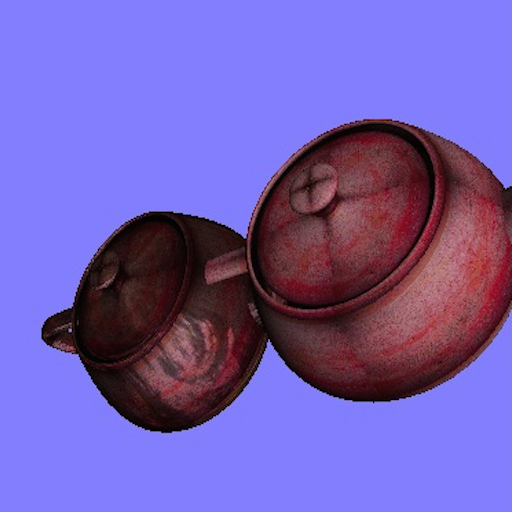
\includegraphics[height=3.5cm]{OGL_texture/mapping_color.png}}&
	\fbox{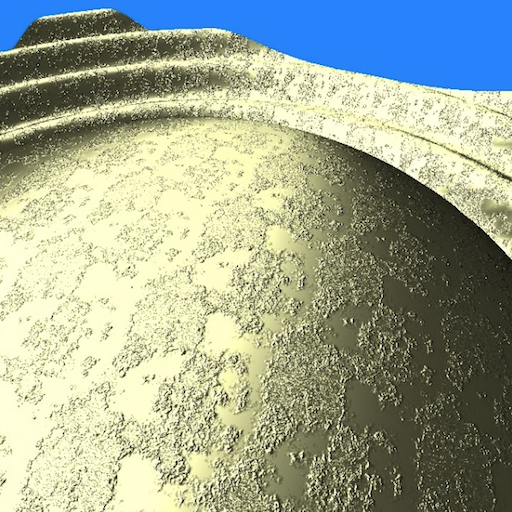
\includegraphics[height=3.5cm]{OGL_texture/mapping_bump.png}}&
	\fbox{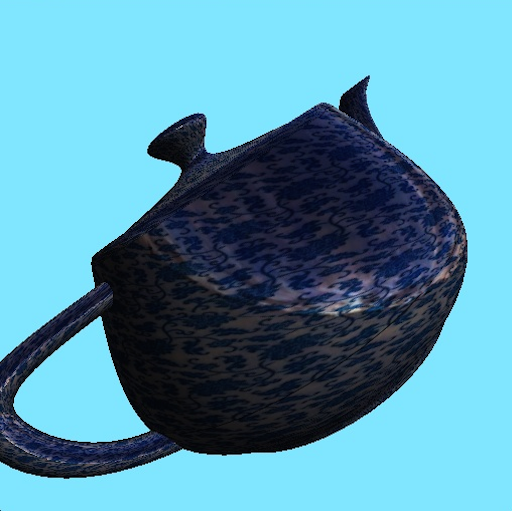
\includegraphics[height=3.5cm]{OGL_texture/mapping_env.png}}\\
(a) 컬러 매핑 & (b) 범프 매핑 & (c) 환경 매핑
\end{tabular}
\end{figure}

\end{frame}
%%%%%%%%%%%%%%%%%%%%%%%%%%%%%%%%%%%%%%%%%%%%%%%%%%%%%%%%%


%%%%%%%%%%%%%%%%%%%%%%%%%%%%%%%%%%%%%%%%%%%%%%%%%%%%%%%%%
\begin{frame}[fragile]{텍스처 매핑의 방법 - 전방 매핑(forward mapping)}

\begin{itemize}
\item 텍스처 매핑의 아이디어는 매우 간단
\item 텍스처 공간에서의 좌표 $(s,t)$를 텍스처 좌표, 물체 표면의 좌표 $(x,y,z)$를 전역공간 좌표라 함
\item 장면을 표현하는 기하공간의 좌표 (x,y,z)는 실수 원소를 가지는 데에 반해 텍스처 공간의 좌표 (s,t)는 정수 원소
\item 하나의 정수 좌표에 의해 얻어지는 텍스처 이미지 상의 한 점을 텍셀(texel)
\item 화면에 그려질 때 화면 좌표계의 한 점을 화소 혹은 픽셀(pixel)
\end{itemize}

매핑이라는 것은 텍스처가 표현하는 정보를 장면을 표현하는 기하 공간의 물체로 옮기면 되므로, 이것을 이런 매핑 함수로 구현할 수 있다.

$$x = {\mathcal X}(s,t), ~ y = {\mathcal Y}(s,t), ~ z={\mathcal Z}(s,t)$$

\end{frame}
%%%%%%%%%%%%%%%%%%%%%%%%%%%%%%%%%%%%%%%%%%%%%%%%%%%%%%%%%


%%%%%%%%%%%%%%%%%%%%%%%%%%%%%%%%%%%%%%%%%%%%%%%%%%%%%%%%%
\begin{frame}[fragile]{후방 매핑(backward mapping)}

\begin{itemize}
\item 전방 매핑: 텍스처 이미지는 정수개의 픽셀로 구성된 텍셀을 객체에 옮겨 놓게 되면 빈 공간이 생길 수 있음
\item 실제 텍스처 매핑은 역방향 매핑(backward mapping)을 수행
\item $s = {\mathcal S}(x,y,z), ~ t = {\mathcal T}(x,y,z)$
\end{itemize}

\begin{figure}[h!]
  \centering
	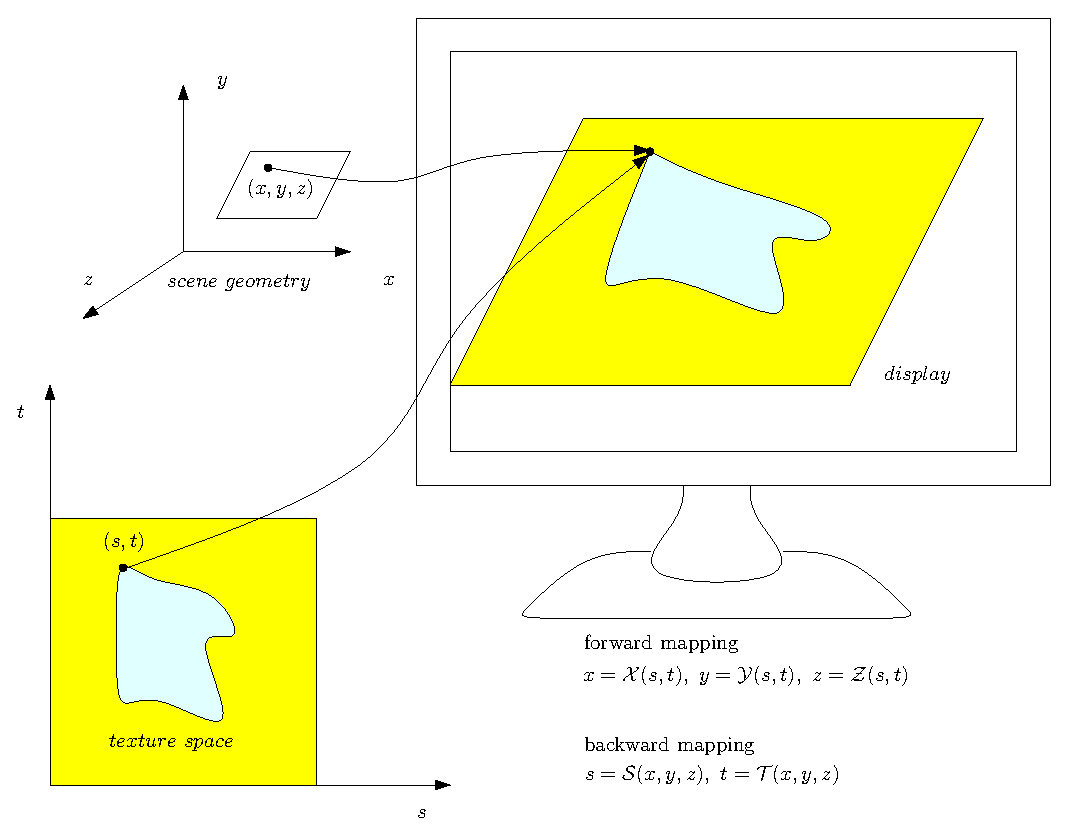
\includegraphics[height=6cm]{OGL_texture/textureMapping.eps}
\end{figure}

\end{frame}
%%%%%%%%%%%%%%%%%%%%%%%%%%%%%%%%%%%%%%%%%%%%%%%%%%%%%%%%%


%%%%%%%%%%%%%%%%%%%%%%%%%%%%%%%%%%%%%%%%%%%%%%%%%%%%%%%%%
\begin{frame}[fragile]{OpenGL을 이용한 텍스처 매핑 구현}

OpenGL에서 텍스처를 적용하는 과정은 다음과 같은 3 개의 단계를 거친다.
\begin{itemize}
\item {\small \sf 텍스처 지정  - 이미지 읽기 혹은 생성, 텍스처 지정, 텍스처 사용 가능하게 하기}
\item {\small \sf 각 정점에 텍스처 좌표 지정 - 매핑 함수는 응용 프로그램의 몫}
\item{\small \sf 텍스처 파라미터 설정 - 래핑(wrapping), 필터링(filtering) 방법 설정}
\end{itemize}

\end{frame}
%%%%%%%%%%%%%%%%%%%%%%%%%%%%%%%%%%%%%%%%%%%%%%%%%%%%%%%%%


%%%%%%%%%%%%%%%%%%%%%%%%%%%%%%%%%%%%%%%%%%%%%%%%%%%%%%%%%
\begin{frame}[fragile]{텍스처 이미지 데이터 만들기}

\lstset{language=C++, escapechar=^} 
\begin{lstlisting}
\begin{lstlisting}
GLubyte myTex[TEXSIZE][TEXSIZE][3];  // ^{\it {\sf TEXSIZE}는 16으로 정의된 것으로 가정하자}^
void CreateTexture(void) {
  for(int i=0;i<TEXSIZE;i++) {
    for(int j=0;j<TEXSIZE;j++) {
       for(int k=0;k<3;k++) {			
          myTex[i][j][k] = (GLubyte) (255*float(rand()\%1000)/999.0);
       } // end k
    } // end j
  } // end i
}
\end{lstlisting}

\end{frame}
%%%%%%%%%%%%%%%%%%%%%%%%%%%%%%%%%%%%%%%%%%%%%%%%%%%%%%%%%


%%%%%%%%%%%%%%%%%%%%%%%%%%%%%%%%%%%%%%%%%%%%%%%%%%%%%%%%%
\begin{frame}[fragile]{OpenGL 텍스처 데이터 생성}

\begin{itemize}
\item 앞의 배열은 이미지를 담고 있을뿐 오픈지엘이 사용할 수 있는 텍스처가 아님
\item 오픈지엘에서 활용할 수 있는 텍스처로 만드는 방법은 {\sf glTexImage2D} 같은 함수를 사용하는 것
\item 다음의 코드는 {\sf glTexImage2D}를 이용하여 앞서 준비한 배열(이미지)를 오픈지엘 텍스처로 만드는 작업을 수행
\end{itemize}

\lstset{language=C++, escapechar=^} 
\begin{lstlisting}
\begin{lstlisting}
void SetupTexture(void) 
{
  glTexImage2D(GL_TEXTURE_2D, 0, GL_RGB, 
            TEXSIZE, TEXSIZE, 0, GL_RGB, 
            GL_UNSIGNED_BYTE, &myTex[0][0][0]);
	
  glTexParameterf(GL_TEXTURE_2D, GL_TEXTURE_WRAP_S, GL_CLAMP);
  glTexParameterf(GL_TEXTURE_2D, GL_TEXTURE_WRAP_T, GL_REPEAT);
  glTexParameterf(GL_TEXTURE_2D, GL_TEXTURE_MAG_FILTER, GL_LINEAR);
  glTexParameterf(GL_TEXTURE_2D, GL_TEXTURE_MIN_FILTER, GL_NEAREST);
  glEnable(GL_TEXTURE_2D);
}
\end{lstlisting}

\end{frame}
%%%%%%%%%%%%%%%%%%%%%%%%%%%%%%%%%%%%%%%%%%%%%%%%%%%%%%%%%


%%%%%%%%%%%%%%%%%%%%%%%%%%%%%%%%%%%%%%%%%%%%%%%%%%%%%%%%%
\begin{frame}[fragile]{{\sf glTexImage2D}의 파라미터}

\begin{itemize}
\item {\sf glTexImage2D}는 2차원 텍스처 ({\sf GL\_TEXTURE\_2D})를 생성하는 것
\item 크기가 {\sf TEXSIZE} $\times$ {\sf TEXSIZE}
\item 각각의 원소가 {\sf GL\_UNSIGNED\_BYTE}임
\item 이미지의 각 원소는 {\sf GL\_RGB} 모드로 저장되어 있음을 알려줌
\end{itemize}

텍스처 파라미터 설정
\begin{itemize}
\item 이어지는 코드는 텍스처 좌표 $s$와 $t$가 [0,1]의 범위를 넘어설 때에 어떻게 할 것인지를 지정
\item {\sf GL\_CLAMP}는 0보다 작거나, 1보다 큰 경우, 각각 0와 1로 취급
\item 1을 넘을 경우 다시 0에서 시작하게 하는 방식은 {\sf GL\_WRAP}
\item {\sf MAG/MIN} 필터는 텍스처가 원래의 크기보다 더 큰 공간으로 가거나, 더 작은 공간으로 갈 때, 보간을 수행하거나({\sf GL\_LINEAR}), 가장 가까운 텍셀을 사용하는({\sf GL\_NEAREST}) 방식을 결정
\item 마지막으로 {\sf GL\_TEXTURE\_2D}를 사용할 수 있도록 glEnable 함수를 이용하여 상태 변경
\end{itemize}


\end{frame}
%%%%%%%%%%%%%%%%%%%%%%%%%%%%%%%%%%%%%%%%%%%%%%%%%%%%%%%%%


%%%%%%%%%%%%%%%%%%%%%%%%%%%%%%%%%%%%%%%%%%%%%%%%%%%%%%%%%
\begin{frame}[fragile]{객체 그리기}

그림을 그리는 것은 다음과 같이 각각의 정점에 텍스처 좌표 $(s,t)$를 지정한다. 
이렇게 정점별로 텍스처 좌표가 지정되면, 폴리곤 내부의 점들의 텍스처 좌표는 선형보간을 통해 결정된다.

\lstset{language=C++, escapechar=^} 
\begin{lstlisting}
void drawAPlane(void) {
  float m=-1;
  float p= 1;
  glBegin(GL_QUADS);
   glTexCoord2f(0, 1);
   glVertex3f(m,p,0); 
   glTexCoord2f(0, 0);
   glVertex3f(m,m,0); 
   glTexCoord2f(1, 0);
   glVertex3f(p,m,0); 
   glTexCoord2f(1, 1);
   glVertex3f(p,p,0);
  glEnd();
}
\end{lstlisting}


\end{frame}
%%%%%%%%%%%%%%%%%%%%%%%%%%%%%%%%%%%%%%%%%%%%%%%%%%%%%%%%%

%%%%%%%%%%%%%%%%%%%%%%%%%%%%%%%%%%%%%%%%%%%%%%%%%%%%%%%%%
\begin{frame}[fragile]{결과 1}

\begin{figure}[h!]
  \centering
	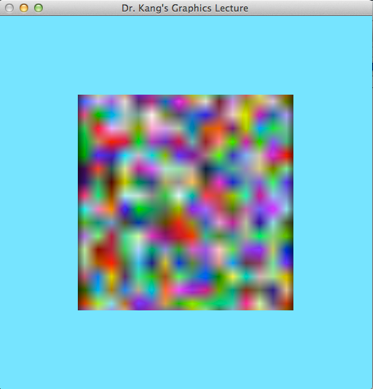
\includegraphics[height=6cm]{OGL_texture/texMap1.png}
\end{figure}


이때 이 이미지가 흐리게 나타나는 이유는 {\sf GL\_TEXTURE\_MAG\_FILTER}를 {\sf GL\_LINEAR}로 
설정했기 때문.


\end{frame}
%%%%%%%%%%%%%%%%%%%%%%%%%%%%%%%%%%%%%%%%%%%%%%%%%%%%%%%%%


%%%%%%%%%%%%%%%%%%%%%%%%%%%%%%%%%%%%%%%%%%%%%%%%%%%%%%%%%
\begin{frame}[fragile]{결과 2}

\begin{figure}[h!]
  \centering
	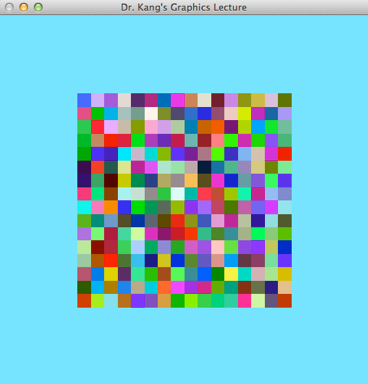
\includegraphics[height=6cm]{OGL_texture/texMap2.png}
\end{figure}

 {\sf GL\_TEXTURE\_MAG\_FILTER}를 {\sf GL\_NEAREST}로 바꾸면 텍셀 값을 보간하지 않고 가장 가까운 값을 그대로 가지고 오기 때문에
원래의 이미지를 또렷하게 확대한 장면을 얻는다.


\end{frame}
%%%%%%%%%%%%%%%%%%%%%%%%%%%%%%%%%%%%%%%%%%%%%%%%%%%%%%%%%


%%%%%%%%%%%%%%%%%%%%%%%%%%%%%%%%%%%%%%%%%%%%%%%%%%%%%%%%%
\begin{frame}[fragile]{결과 3}

텍스처를 사용한 상태에서 {\sf glutSolidTeapot(...)}을 호출하면 다음과 같이 그려진다. 이때 앞서 다룬 조명을 제대로 설정해야 주전자가 음영을 갖고 그려진다.

\begin{figure}[h!]
  \centering
	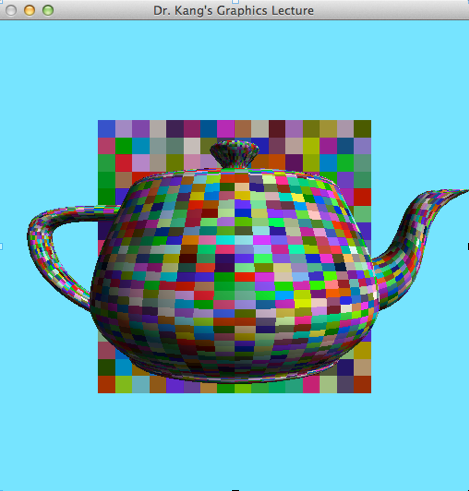
\includegraphics[height=6cm]{OGL_texture/texMap3.png}
\end{figure}


\end{frame}
%%%%%%%%%%%%%%%%%%%%%%%%%%%%%%%%%%%%%%%%%%%%%%%%%%%%%%%%%


%%%%%%%%%%%%%%%%%%%%%%%%%%%%%%%%%%%%%%%%%%%%%%%%%%%%%%%%%
\begin{frame}[fragile]{이미지 읽어 텍스처로 사용하기}

\begin{itemize}
\item 이미지 파일을 직접 절차적으로 생성하는 방식은 다양한 텍스처를 손쉽게 만들 수 있는 방법은 아님
\item 효율적인 방법은 이미지 편집 도구를 이용하여 텍스처 이미지를 만들고, 이를 불러서 사용하는 것
\item 이미지 파일을 다루는 코드를 작성해야 함
\item 우리는 이를 직접 작성하지 않고, 이미 만들어져 공개된 소스를 활용
\item 이미지를 읽어들이는 방법은 STB Image 라이브러리를 사용할 것이며, 이 라이브러리는 다음 URL에서 구할 수 있음
\end{itemize}

\begin{verbatim}
http://www.nothings.org/stb_image.c
\end{verbatim}

\end{frame}
%%%%%%%%%%%%%%%%%%%%%%%%%%%%%%%%%%%%%%%%%%%%%%%%%%%%%%%%%

%%%%%%%%%%%%%%%%%%%%%%%%%%%%%%%%%%%%%%%%%%%%%%%%%%%%%%%%%
\begin{frame}[fragile]{STB Image 라이브러리로 이미지 읽기}

\lstset{language=C++, escapechar=^} 
\begin{lstlisting}
int width, height, bitsPerPixel;
unsigned char *data = stbi_load("cosmos.jpg", &width, &height, 
                             &bitsPerPixel, 0);
glGenTextures(1, &texture);
glBindTexture(GL_TEXTURE_2D, texture);
glTexImage2D(GL_TEXTURE_2D, 0, GL_RGB, width, height, 0, 
              GL_RGB, GL_UNSIGNED_BYTE, data);
\end{lstlisting}

\end{frame}
%%%%%%%%%%%%%%%%%%%%%%%%%%%%%%%%%%%%%%%%%%%%%%%%%%%%%%%%%


%%%%%%%%%%%%%%%%%%%%%%%%%%%%%%%%%%%%%%%%%%%%%%%%%%%%%%%%%
\begin{frame}[fragile]{이미지를 활용한 텍스처 생성}

\lstset{language=C++, escapechar=^} 
\begin{lstlisting}
^{\sf \color{red} texture.h}^
...
GLuint setTexture(char *filename);
...


^{\sf \color{red} texture.cpp}^
...
#include "STBImage.h"
GLuint setTexture(char *filename) {
	GLuint texture;
	int width, height, bitsPerPixel;
	unsigned char *data = stbi_load(filename, &width, &height, &bitsPerPixel, 0);
	glGenTextures(1, &texture);
	glBindTexture(GL_TEXTURE_2D, texture);
	glTexImage2D(GL_TEXTURE_2D, 0, GL_RGB,
				width, height, 0, GL_RGB, GL_UNSIGNED_BYTE, data);

	glTexParameterf(GL_TEXTURE_2D, 		GL_TEXTURE_WRAP_S, GL_REPEAT);
	glTexParameterf(GL_TEXTURE_2D, 		GL_TEXTURE_WRAP_T, GL_REPEAT);
	glTexParameterf(GL_TEXTURE_2D, 		GL_TEXTURE_MAG_FILTER, GL_LINEAR);
	glTexParameterf(GL_TEXTURE_2D, 		GL_TEXTURE_MIN_FILTER, GL_LINEAR);
	glEnable(GL_TEXTURE_2D);
	return texture;
}
\end{lstlisting}

\end{frame}
%%%%%%%%%%%%%%%%%%%%%%%%%%%%%%%%%%%%%%%%%%%%%%%%%%%%%%%%%

%%%%%%%%%%%%%%%%%%%%%%%%%%%%%%%%%%%%%%%%%%%%%%%%%%%%%%%%%
\begin{frame}[fragile]{텍스처 적용하기}

\lstset{language=C++, escapechar=^} 
\begin{lstlisting}
void display() {
  glClear(GL_COLOR_BUFFER_BIT|GL_DEPTH_BUFFER_BIT);
  glMatrixMode(GL_MODELVIEW);
  glLoadIdentity();
  gluLookAt(0, 0, 3, 0, 0, 0, 0, 1, 0);
  LightPositioning();
  drawAPlane();
  glutSolidTeapot(1.0);
  glutSwapBuffers();
}
\end{lstlisting}

\end{frame}
%%%%%%%%%%%%%%%%%%%%%%%%%%%%%%%%%%%%%%%%%%%%%%%%%%%%%%%%%


%%%%%%%%%%%%%%%%%%%%%%%%%%%%%%%%%%%%%%%%%%%%%%%%%%%%%%%%%
\begin{frame}[fragile]{텍스처 적용 결과}

\begin{figure}[h!]
  \centering
	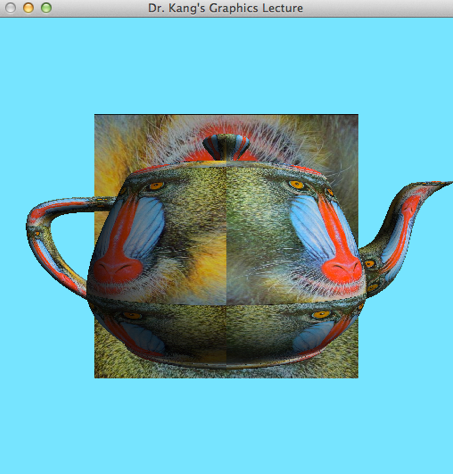
\includegraphics[height=7cm]{OGL_texture/textureImageApplied.png}
\end{figure}

\end{frame}
%%%%%%%%%%%%%%%%%%%%%%%%%%%%%%%%%%%%%%%%%%%%%%%%%%%%%%%%%


%%%%%%%%%%%%%%%%%%%%%%%%%%%%%%%%%%%%%%%%%%%%%%%%%%%%%%%%%
\begin{frame}[fragile]{복수의 텍스처 사용 - 텍스처 바인딩(binding)}

\begin{itemize}
\item 두 개의 텍스처를 다룰 수 있도록 텍스처를 가리키는 번호를 저장할 두 개의 변수 사용
\item 각각의 텍스처를 사용해야 할 때마다, 원하는 텍스처를 지정
\item 텍스처 바인딩(texture binding)
\end{itemize}

\lstset{language=C++, escapechar=^} 
\begin{lstlisting}
  GLuint tex1, tex2;
  tex1 = setTexture("baboon.jpg");
  tex2 = setTexture("cartoon.jpg");
  glBindTexture(GL_TEXTURE_2D, tex1);
  drawAPlane();
  glBindTexture(GL_TEXTURE_2D, tex2);
  glutSolidTeapot(0.75);
\end{lstlisting}

\end{frame}
%%%%%%%%%%%%%%%%%%%%%%%%%%%%%%%%%%%%%%%%%%%%%%%%%%%%%%%%%


%%%%%%%%%%%%%%%%%%%%%%%%%%%%%%%%%%%%%%%%%%%%%%%%%%%%%%%%%
\begin{frame}[fragile]{텍스처 좌표 자동생성}

\begin{itemize}
\item 텍스처 좌표를 자동으로 생성할 수 있다면, 일일히 텍스처 좌표를 지정하지 않아도 됨
\item 환경 매핑과 같은 경우에 이 기법이 유용하게 사용
\item OpenGL이 자동으로 각 정점의 텍스처 좌표를 결정하는 방법이 있음
\item 이를 위해서는 아래와 같이 자동 생성이 가능하도록 해야 함
\end{itemize}

\lstset{language=C++, escapechar=^} 
\begin{lstlisting}
glEnable(GL_TEXTURE_GEN_S);
glEnable(GL_TEXTURE_GEN_T);
\end{lstlisting}

\end{frame}
%%%%%%%%%%%%%%%%%%%%%%%%%%%%%%%%%%%%%%%%%%%%%%%%%%%%%%%%%


%%%%%%%%%%%%%%%%%%%%%%%%%%%%%%%%%%%%%%%%%%%%%%%%%%%%%%%%%
\begin{frame}[fragile]{{\sf GL\_EYE\_LINEAR}}

\lstset{language=C++} 
\begin{lstlisting}
glTexGenf(GL_S, GL_TEXTURE_GEN_MODE, 	GL_EYE_LINEAR);
glTexGenf(GL_T, GL_TEXTURE_GEN_MODE, 	GL_EYE_LINEAR);
\end{lstlisting}

\begin{figure}[h!]
  \centering
	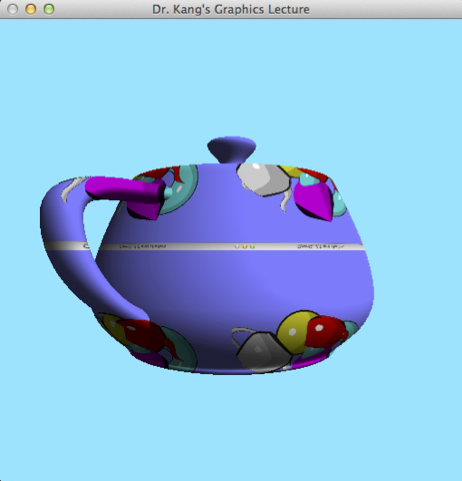
\includegraphics[height=6cm]{OGL_texture/eyeLinear1.png}
	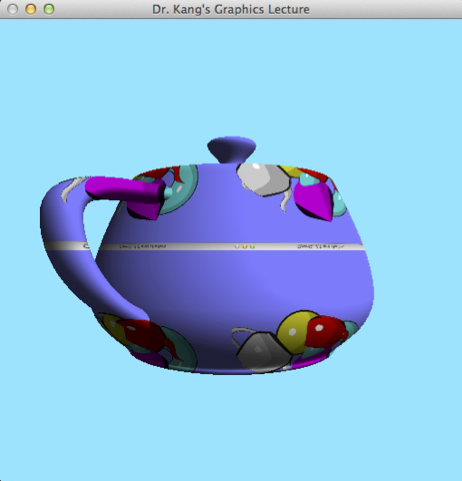
\includegraphics[height=6cm]{OGL_texture/eyeLinear2.png}
\end{figure}

\end{frame}
%%%%%%%%%%%%%%%%%%%%%%%%%%%%%%%%%%%%%%%%%%%%%%%%%%%%%%%%%

%%%%%%%%%%%%%%%%%%%%%%%%%%%%%%%%%%%%%%%%%%%%%%%%%%%%%%%%%
\begin{frame}[fragile]{{\sf GL\_OBJECT\_LINEAR}}

\lstset{language=C++} 
\begin{lstlisting}
glTexGenf(GL_S, GL_TEXTURE_GEN_MODE, 	GL_OBJECT_LINEAR);
glTexGenf(GL_T, GL_TEXTURE_GEN_MODE, 	GL_OBJECT_LINEAR);
\end{lstlisting}

\begin{figure}[h!]
  \centering
	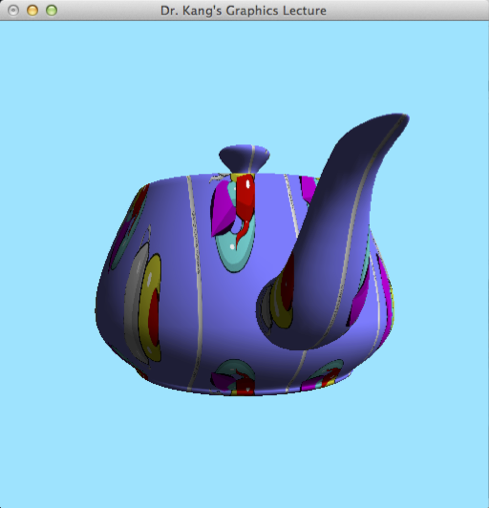
\includegraphics[height=6cm]{OGL_texture/objLinear1.png}
	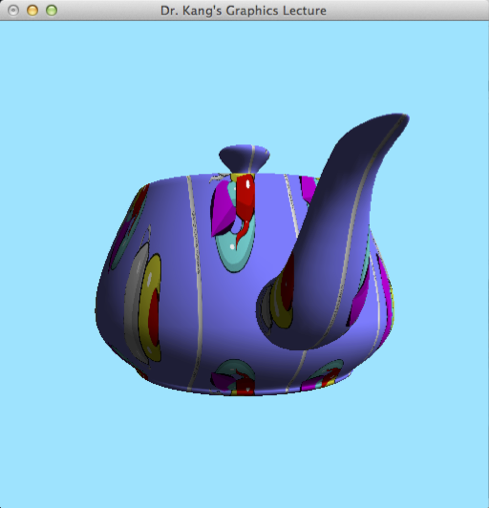
\includegraphics[height=6cm]{OGL_texture/objLinear2.png}
\end{figure}

\end{frame}
%%%%%%%%%%%%%%%%%%%%%%%%%%%%%%%%%%%%%%%%%%%%%%%%%%%%%%%%%


%%%%%%%%%%%%%%%%%%%%%%%%%%%%%%%%%%%%%%%%%%%%%%%%%%%%%%%%%
\begin{frame}[fragile]{{\sf GL\_SPHEREMAP}}

\lstset{language=C++} 
\begin{lstlisting}
glTexGenf(GL_S, GL_TEXTURE_GEN_MODE, GL_SPHERE_MAP);
glTexGenf(GL_T, GL_TEXTURE_GEN_MODE, GL_SPHERE_MAP);
\end{lstlisting}

\begin{figure}[h!]
  \centering
	\begin{tabular}{cc}\\ \hline
	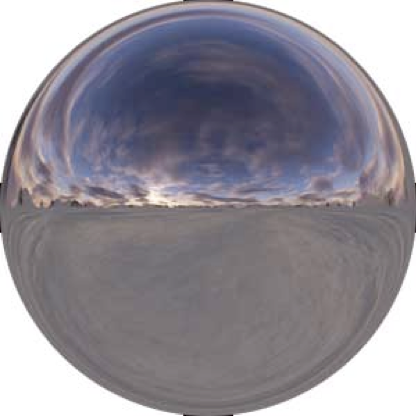
\includegraphics[height=6cm]{OGL_texture/sphereMap.png} &
	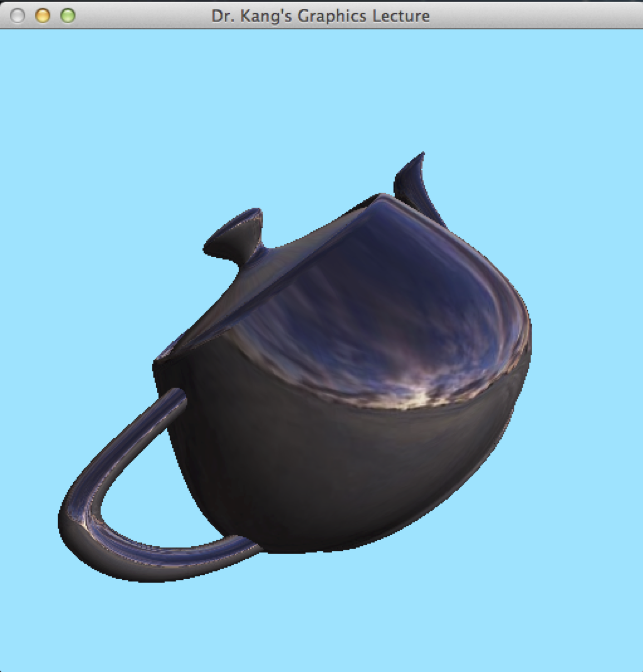
\includegraphics[height=6cm]{OGL_texture/sphereMapped.png} \\
	(a) 구면 맵의 예 & (b) 구면 맵이 적용된 결과
	\end{tabular}
\end{figure}

\end{frame}
%%%%%%%%%%%%%%%%%%%%%%%%%%%%%%%%%%%%%%%%%%%%%%%%%%%%%%%%%


%%%%%%%%%%%%%%%%%%%%%%%%%%%%%%%%%%%%%%%%%%%%%%%%%%%%%%%%%
\begin{frame}[fragile]{텍스처 좌표 자동생성 비교}

\lstset{language=C++} 
\begin{lstlisting}
	glTranslated(-0.5, 0.0, 0.0);
	glBindTexture(GL_TEXTURE_2D, tex1);
	glEnable(GL_TEXTURE_GEN_S); glEnable(GL_TEXTURE_GEN_T);
	glTexGenf(GL_S, GL_TEXTURE_GEN_MODE, 	GL_EYE_LINEAR);
	glTexGenf(GL_T, GL_TEXTURE_GEN_MODE, 	GL_EYE_LINEAR);
	glutSolidTeapot(0.6);
	glTranslated(0.5, 0.0, 0.0);
	glEnable(GL_TEXTURE_GEN_S); glEnable(GL_TEXTURE_GEN_T);
	glTexGenf(GL_S, GL_TEXTURE_GEN_MODE, 	GL_OBJECT_LINEAR);
	glTexGenf(GL_T, GL_TEXTURE_GEN_MODE,	GL_OBJECT_LINEAR);
	glutSolidTeapot(0.6);
	glTranslated(0.5, 0.0, 0.0);
	glBindTexture(GL_TEXTURE_2D, tex2);
	glEnable(GL_TEXTURE_GEN_S); glEnable(GL_TEXTURE_GEN_T);
	glTexGenf(GL_S, GL_TEXTURE_GEN_MODE,	GL_SPHERE_MAP);
	glTexGenf(GL_T, GL_TEXTURE_GEN_MODE, 	GL_SPHERE_MAP);
	glutSolidTeapot(0.6);
\end{lstlisting}

\end{frame}
%%%%%%%%%%%%%%%%%%%%%%%%%%%%%%%%%%%%%%%%%%%%%%%%%%%%%%%%%

%%%%%%%%%%%%%%%%%%%%%%%%%%%%%%%%%%%%%%%%%%%%%%%%%%%%%%%%%
\begin{frame}[fragile]{텍스처 좌표 자동생성 비교}

\begin{figure}[h!]
  \centering
	\begin{tabular}{c}
	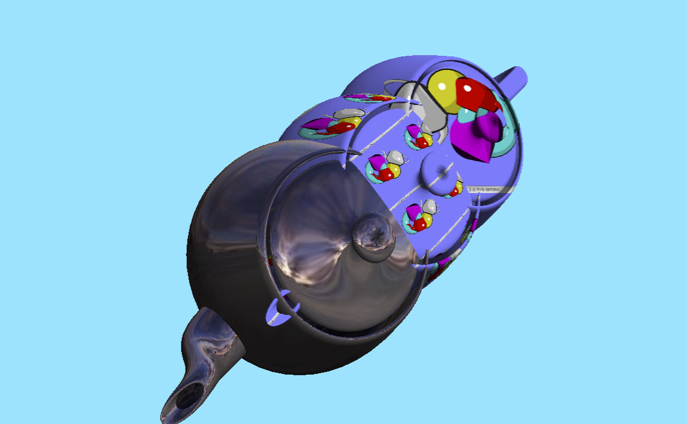
\includegraphics[width=9cm]{OGL_texture/mappingComparison2.png} 
	\end{tabular}
\end{figure}

\end{frame}
%%%%%%%%%%%%%%%%%%%%%%%%%%%%%%%%%%%%%%%%%%%%%%%%%%%%%%%%%




\end{document}



